\documentclass[12pt]{article}

\usepackage{geometry}  
\geometry{letterpaper}
\usepackage[usenames,dvipsnames,svgnames,table]{xcolor}
\usepackage[T1]{fontenc}
%\usepackage{eulervm}
%\usepackage{graphicx}
\usepackage{epstopdf}
\usepackage{tikz}
\usepackage{pgfplots}
\usepackage{pgfplotstable}
\usepackage{amsmath}
\usepackage{amssymb}
%\usepackage{booktabs}
%\usepackage{array}
\usepackage{colortbl}
\usepackage{booktabs}
\usetikzlibrary{trees,decorations,arrows,automata,positioning,plotmarks,
	shapes,backgrounds,petri,fit}

\usepackage{graphicx}
% !TEX root = ./active_learning.tex

\newcommand{\set}[1]{\left\{ #1 \right\}}
\newcommand{\note}[1]{{\color{Green} NB: #1}}
\newcommand{\vek}[1]{{\bf #1}}
\newcommand{\sigmoid}[1]{{\sigma \left(#1\right)}}
\newcommand{\ie}{i.e.\ }
\newcommand{\prob}[1]{{P(#1)}}
\newcommand{\prior}[1]{{\pi(#1)}}
\newcommand{\ud}{\,\mathrm{d}}
\newcommand{\data}{\,\mathcal{D}}
\newcommand{\params}{\theta}
\newcommand{\inp}{\vek x}
\newcommand{\outp}{\vek y}
\newcommand{\expect}[2]{\mathbb{E}_{#1 \sim \prob{#2}}}
\newcommand{\utility}{\mathcal{U}}
\newcommand{\model}{\mathcal{M}}
\newcommand{\xconv}{x_\infty}

\textwidth430pt
\textheight600pt
\topmargin0pt
\oddsidemargin-20pt
\usepackage{lineno}
\linenumbers
\usepackage{setspace}
\usepackage{wrapfig}
\usepackage{titling}
\usepackage{siunitx}


%\usepackage[usenames,dvipsnames]{xcolor}
\usepackage[usenames,dvipsnames,svgnames,table]{xcolor}
\usepackage[T1]{fontenc}
%\usepackage{eulervm}
%\usepackage{graphicx}
\usepackage{epstopdf}
\usepackage{amsmath}
\usepackage{amssymb}
%\usepackage{booktabs}
%\usepackage{array}
\usepackage{colortbl}
\usepackage{booktabs}	
\usepackage{graphicx}% Include figure files
\usepackage{dcolumn}% Align table columns on decimal point
\usepackage{bm}% bold math
\usepackage{hyperref}% add hypertext capabilities
\usepackage{verbatim}
\usepackage{color}
\usepackage{pifont}
\usepackage{bbold}
\usepackage{breqn}
\usepackage{subcaption}

\usepackage{amsmath}
\usepackage[capitalise]{cleveref}

\begin{document}

\doublespacing

\title{Active Learning -- CCCN 2016, Lisbon}

\author{Laura Driscoll, Simon Weber, Peter Zatka-Haas}
\date{\today}

\setlength{\droptitle}{-10em}

\maketitle

% !TEX root = ./active_learning.tex

\section*{General introduction} % (fold)
\label{sec:general_introduction}

\subsection{Uncertainties in determining model parameters from data} % (fold)
\label{sub:uncertainties_in_determining_model_parameters_from_data}
\begin{itemize}
	\item \textbf{Parameter uncertainty:}
	Observed data sets are finite. Therefore it is impossible to determine the parameters of a model precisely. \\
	In our example we can't be confident about the psychometric curve if we have few data points.
	\item \textbf{Inherent uncertainty:}
	Typically there is noise in observing the data. In other words, there is randomness in the data that is not explained by the model.
	Inherent uncertainty is also called \textbf{observation noise}. \\
	In our example the inherent uncertainty is high at low contrast differences.
\end{itemize}
% subsection uncertainties_in_determining_model_parameters_from_data (end)

Notation: \\
Data $\data$. New data $\data^*$. Parameters $\params$. Input $\inp$. Output $\outp$. Model $\model$. \\
\note{We might not mention the $\model$ explicitly in all the probabilities}.

We are interested in the posterior probability of the model parameters given the data
\begin{align}\label{eq:posterior}
	\prob{\params | \data, \model} = \frac{\prob{\data | \params, \model} \prior{\params | \model}}{\prob{\data | \model}}
\end{align}
The posterior reflects the parameters for which the model best describes the data and the underlying uncertainty (parameter uncertainty).
Another probability that occurs frequently in the following is the \emph{predictive distribution}.
The predictive distribution is the probability $\prob{\data^* | \data, \model}$ of observing a new data point $\data^*$ given the old data $\data$ and a model $\model$.
\begin{align}
	\prob{\data^* | \data, \model}
	&= \int \ud \params
		\prob{\data^*, \params | \data, \model} \\
	&= \int \ud \params
		\prob{\data^* | \data, \params, \model}
		\prob{\params | \data, \model} \\
	&= \int \ud \params
		\underbrace{
		\prob{\data^* | \params, \model}}_{\text{inherent uncertainty}}
		\underbrace{
		\prob{\params | \data, \model}}_{\text{parameter uncertainty}} \,, \label{eq:predictive_distribution}
\end{align}
where in the last step we used $\prob{\data^* | \data, \model, \params} = \prob{\data^* | \model, \params}$, because the new data should depend only on the model and the parameters and not on the collected data. That is, we assume that the model captures all the structure in the data. This assumption is typical for Bayesian inference. Note how \cref{eq:predictive_distribution} contains both aforementioned uncertainties. 

It is typically desirable to have little uncertainty in the posterior. The amount of uncertainty can be measured by the entropy
\begin{align}
	H[\prob{\params | \data}] =
	- \expect{\params}{\params | \data}
	\log \prob{\params | \data}
\end{align}
In the psychophysics experiment that we conduct, the data is comprised of stimulus-response pairs. We can choose the stimulus $\inp$ and observe the response $\outp$. Say we have collected some stimulus-response pairs already (represented with $\data$). The goal is to choose the next stimulus $\inp$ such that the uncertainty in the posterior is decreased. In other words, we would like to choose $\inp$ such that the corresponding decrease in entropy
\begin{align}
	H[p(\params | \data)] - H[p(\params | \data, \inp, \outp)]
\end{align}
is maximal. But we don't know the answer $\outp$ that we are going to get. We can only maximize the decrease in expected posterior entropy:
\begin{align}
	\utility(\inp)
	= H[p(\params | \data)]
	- \expect{\outp}{\outp | \inp, \data} H[\prob{\params | \data, \inp, \outp}] \,,
\end{align}
which corresponds to minimizing the second term. This is called posterior entropy minimization.
We can get an alternative formulation by noting that
\begin{align}
	\utility(\inp)
	&= I[\params, \outp | \data, \inp] \\
	&=
	\underbrace{
	H[\prob{\outp | \inp, \data}]}_{\text{marginal entropy}}
	-
	\underbrace{
	\expect{\params}{\params | \data} H[\prob{\outp | \inp, \params}]}_{\text{expected conditional entropy}}
	\,,
\end{align}
where $I$ is the mutual information, which is symmetric in its arguments. Writing it this way allows for a different interpretation of the utility function $\utility(\inp)$.
The first term (the marginal entropy) is the entropy of the predictive distribution:
\begin{align}
	\entropy{\prob{\outp | \inp, \data}} = \entropy{\int \ud \params' \prob{\outp | \inp, \params'} \prob{\params' | \data}} \,.
\end{align}
This term reflects the parameter uncertainty.
It should be large, because we want to choose an input $\inp$ for which the parameters $\params'$ disagree about the output $\outp$. If they would all agree, we would not get useful information about which parameters are better than others.
More precisely, if for different $\params'$ different $\outp$ are likely, than the integral results in a non-vanishing probability for many values of $\outp$. We thus get a high entropy.

The second term (the expected conditional entropy) is:
\begin{align}
	\expect{\params}{\params | \data} H[\prob{\outp | \inp, \params}]
	= \int \ud \params' \prob{\params'|\data} \entropy{\prob{\outp | \inp, \params'}} \,.
\end{align} 
This term reflects the inherent uncertainty because it is high if all $\outp$ are equally probable for the given parameter $\params'$. The term should be small. This makes sense, because if the prediction of the output $\outp$ given by the model parameters $\params'$ is very uncertain at the input $\inp$, we learn very little about the choice of the parameters after we observed the response. We thus should choose an $\inp$ for which the parameter sets $\params'$ typically make a confident prediction of the response.
Now $H[\prob{\outp | \inp, \data}]$ should be large, which makes sense, because we should choose an input.

\note{Copied from Houlsby thesis: In other words, we seek the input $\inp$ for which the parameters under the posterior make confident predictions [term 2], but these predictions are highly diverse [term 1]. That [term 1] is, the parameters disagree about the output $\outp$, hence this formulation is named Bayesian Active Learning by Disagreement (BALD).
}

\begin{figure}
\centering
  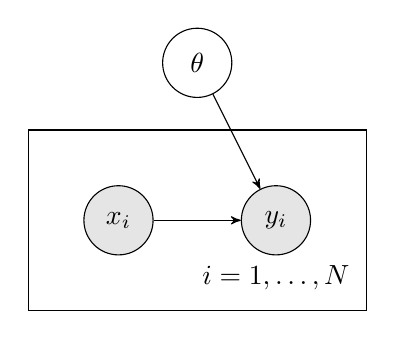
\begin{tikzpicture}[auto, bend angle=10, ->, >=stealth', initial text=]
	\node[state]	(t) at (1, 2)  {$ \params $};
	\node[state, fill = black!10]	(x) at (0, 0)  {$ x_i $};
	\node[state, fill = black!10]	(y) at (2, 0) [label=below:{$i=1,\dots,N$}] {$ y_i $};
	\path (t) edge         node {} (y);
	\path (x) edge         node {} (y);
	\node[rectangle, draw=black!100, inner sep=7mm, fit= (x) (y)] {};	
  \end{tikzpicture}
  \caption{Graphical model. White notes indicate latent (unobserved) variables and shaded notes denote observed variables. The stimulus $x$ is independent of the parameters $\params$. Adapted from Houlsby thesis.}
\end{figure}
% subsection general_introduction (end)
% !TEX root = ./active_learning.tex

\section{Experiment} % (fold)
\label{sec:experiment}

We show two gratings to participants. The frequency of the grating is fixed. The orientation of both gratings is the same but varied in each trial to avoid afterimages. One grating is always of the same contrast level, but the side is chosen at random. We vary the contrast of the other grating.
We characterize the difference in contrast between the grating that is shown on the left and the grating that is shown on the right with $x$. For negative $x$ the grating on the left is of higher contrast, for positive $x$ the stimulus on the right is of higher contrast. If we denote the fixed baseline contrast with $x_b$, then the value of $x$ is in the range $[-(1-x_b), (1-x_b)]$.

We chose the presented $x$ according to different strategies and record the answers (left $L$, or right $R$) of the participants when the decide on which side the grating with higher contrast is shown.

\subsection{Choosing the presented stimulus} % (fold)
\label{sub:choosing_the_presented_stimulus}
We assume a prior $\prior{\params}$ where $\params  = \set{w_0, w_1, \lambda}$ is a set of parameters that describe our model.
As the model $\model$ we use a sigmoid function
\begin{align}
	\sigmoid{\params, x} = \lambda / 2 + \frac{1-\lambda / 2}{1 + \exp[-w_1(x - w_0)]} \,,
\end{align}
where $\lambda$ is the lapse rate. The lapse rate accounts for wrong answers that are not because the task was to difficult, but because the participant hit mistakenly hits the wrong button.
\note{We drop the model $\model$ in all the subsequent probabilities. Whenever we use $\params$ we mean the parameters together with the sigmoid model}.
We collect data $N$ data points by presenting a stimulus $x \in [-1.0, 1.0]$ and observing a binary response $y \in \set{0, 1}$:
\begin{align}
	 \data = \set{(x_1, y_1), \dots, (x_N, y_N)} \equiv (X^N, Y^N)
\end{align}
\note{We drop the $N$, if it is not needed to dissociated the steps.}
The likelihood of the parameters $\params$ given the data $D$ is given by
\begin{align}
	\prob{Y^N | \params, X^N}
	&= \prod_{i=1}^N \prob{y_i | \params, x_i} \\
	&= \prod_{i=1}^N \sigmoid{\params, x}^{y_i}
		\left( 1 - \sigmoid{\params, x} \right)^{1-y_i}
\end{align}
\note{The stimuli $x$ are not considered part of the data, because we have control over it}
The posterior probability of the parameters $\vek w$ is
\begin{align}
	\prob{\params | X, Y} = \frac{\prob{Y | \params, X} \prior{\params}}{\prob{Y | X}}
\end{align}
The denominator, \ie the marginal likelihood, is computed by taking the integral over all hypotheses:
\begin{align}
	\prob{Y | X} = \int \prob{Y | \params', X} \prior{\params'} \ud \params'
\end{align}
The goal is to get a posterior $\prob{\vek w | X, Y}$ that is of low uncertainty. We use entropy as a measure of the current uncertainty of our estimation of $\params$. By \emph{current} we mean that we use the data $\data$ we have discovered in the $N$ steps until now. The new data points are labeled $x, y$.
\begin{align}
	H[\prob{\params | \data}] = - \int \prob{\params' | \data} \log[\prob{\params' | \data}] \ud \params' \,.
\end{align}
In principle we would now like to choose our next stimulus $x$ such that it minimizes the resulting entropy $H(\vek w | X_N, Y_N, x, y)$, but we do not know what $y$ is going to be. So we want to find the $x$ that minimizes the mean:
\begin{align}
	H[\prob{\vek w | \data, x, y = 0}] ~
	\prob{y = 0 | \data, x} \\
	&+
	H[\prob{\vek w | \data, x, y = 1}] ~
	\prob{y = 1 | \data, x} \,.
\end{align}
Here $\prob{y = 0/1 | \data, x}$ is called the \emph{predictive distribution}. Determining them again requires an integral over the hypotheses:
\begin{align}
	\prob{y = 0/1 | \data, x}
	= \int \prob{y = 0/1 | \params, x} \prob{\params | \data} \ud \params
\end{align}

\note{The above is the direct approach without using BALD learning}.

Instead we should use BALD learning and find the $x$ that maximizes:
\begin{align}
	\utility(x) = H[\prob{y | \data, x}]
	- \expect{\params}{\params | \data} H[\prob{y | \params, x}] \,.
\end{align}

\subsection{Humans} % (fold)
\label{sub:humans}
Here the contrast difference $x$ is chosen by a human. They can select every possible value for $x$. To help them they

% subsection humans (end)

% subsection choosing_the_presented_stimulus (end)

% section experiment (end)


% !TEX root = ./active_learning.tex

\section{Approximations} % (fold)
\label{sec:approximations}
We need to determine $K(x)$ for all $x$ values that we consider as worthwhile new stimuli. This can be many values and doing the involved integrals over posteriors is costly.
There are several ways to deal with this problem.

\subsection{Restricting the tested stimuli} % (fold)
\label{sub:restricting_the_tested_stimuli}
We need to discretize the $x$ anyways. We choose values.

\subsection{Approximating the posterior} % (fold)
 \label{sub:approximating_the_posterior}
We often determine the mean of a function over the posterior distribution. This is computationally expensive, in particular for large parameter spaces.
If we take samples of the posterior and approximate the integrals by smaller sums over the samples, we can save computation time. To get good samples from the posterior distribution we use the Metropolis-Hastings algorithm as an implementation of Markov Chain Monte Carlo integration.
As a proposal distribution $Q(x;x')$ we choose a multi variate normal distribution which determines the random walk that samples from the posterior.
 % subsection approximating_the_posterior (end) 

% subsection restricting_the_tested_stimuli (end)
% section approximations (end)
% !TEX root = ./active_learning.tex
\section{Paradox of ladder stimulus presentation} % (fold)
\label{sec:paradox_of_ladder_stimulus_presentation}

Assume a stimulus range from $-a$ to $a$. Imagine we present stimuli in the following way:
\begin{itemize}
	\item We present the first at the center $(x_1=0)$ and record the answer $y_1$
	\item For the $n$-th stimulus ($n>1$) we take
	\begin{align}
		x_n = x_{n-1} + (-1)^{y_{n-1}} \frac{a}{2^{n-1}}
	\end{align}
\end{itemize}
For $N \to \infty$, this leads to a distribution of data points that seems to be best fitted by a step function.
When we collect data this way, we know that it will always lead to a distribution that looks this way and we know that we should not conclude that the underlying psychometric function should have a steep step.
If, however, someone would present us this data and claim that it was obtained without using the ladder algorithm above, we might be tempted to conclude that the underlying psychometric curve is very steep. This is paradoxical, because the likelihood principle claims that the data is all we need to determine our parameter. It should not matter how the data was obtained.

The solution of this paradox is that we should not conclude a step function in neither of the two cases. Instead the posterior suggests that all sigmoids that cross $y^* = \frac{\#\text{ of response 1 around } \xconv}{\#\text{ of response 0 around } \xconv}$ at the stimulus value $\xconv$ to which the ladder method converges are equally probable. \note{'around' is not properly defined here, but it can't be $\xconv$ precisely, because it is never reached. It should be some $\varepsilon$-ball.}
With our parameterization this is the set of sigmoids for which
\begin{align}\label{eq:paradox}
 w_0 = -\xconv w_1 + c \,,	
\end{align}
where $c > 0$ if $y^* > 1/2$, $c = 0$ if $y^* = 1/2$ and $c < 0$ if $y^* < 1/2$.
So for $N \to \infty$ the posterior $\prob{w_0, w_1 | \data}$ turns into a line that is characterized by \cref{eq:paradox}. \\
Marginalizing over the threshold value $w_0$ leads to a flat posterior for the slope $\prob{w_1 | \data}$. This shows that all slopes are equally likely and Bayesian inference does not conclude a step function.
% section paradox_of_ladder_stimulus_presentation (end)


\newpage
\bibliographystyle{ieeetr} 
\bibliography{references}

\end{document}  